\section{Confidence Intervals, Significance Levels, and $p$-values}

\begin{figure}
	\centering
	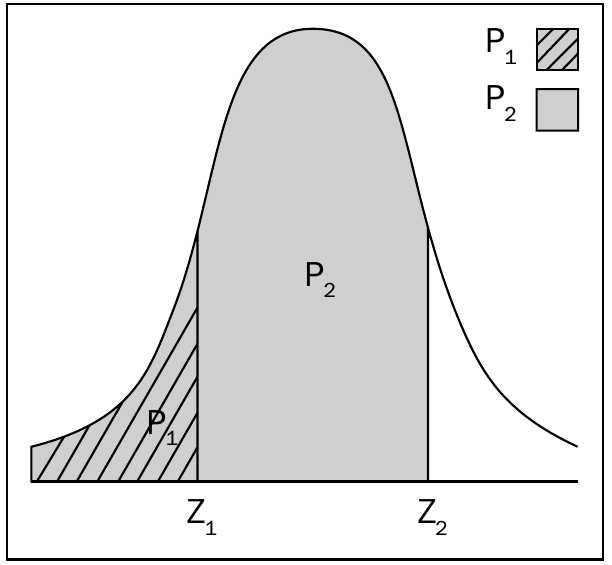
\includegraphics[height=5cm,keepaspectratio=true]{./images/kum0401.png}
	% kum0401.png: 0x0 pixel, 300dpi, 0.00x0.00 cm, bb=
	\caption{A typical normal distribution with $p$-values.}
	\label{fig:3.7.3}
\end{figure}



Suppose that $Z_{1}$ and $Z_{2}$ are two $Z$-statistics corresponding to two values of a random variable, and $p_{1}$ and $p_{2}$ are the areas enclosed by the density curve to the right of those values.

In other words,
\begin{align}
	P(X>Z_{1})=p_{1}\\
	P(X>Z_{2})=p_{2}
\end{align}



Then, we can define an interval in which to find the value of a random variable, which we will call a \emph{confidence interval.}


For example, for a normal distribution with mean $\mu$ and standard deviation $\sigma,$ the value of the random variable will lie in the \emph{interval} $[\mu-3\sigma,\mu+3\sigma]$ with a \emph{confidence} (probability) of $99\%.$


For any \emph{estimator} (random variable) having a normal distribution, one can define a confidence interval if we decide on the confidence level or probability.


We can think of \emph{confidence intervals} as the threshold of accepted values to maintain that the \emph{null hypothesis} is true.


If the value of the estimator lives within this range, it will be statistically correct to state that the null hypothesis is correct.


To define a confidence interval, one must first define a \emph{confidence level (or probability).} This probability needs to be set by the researcher depending on the context.


Let us say that this probability is $p$. In general, we will use the \emph{significance level}
\begin{align}
	\beta = 1-p,
\end{align}
which represents the probability that the null hypothesis is not correct. 

$\beta$ is defined by the researcher and is typically in the range of $0.01$ to $0.1$.



An important concept to learn here is the \emph{probability value} or simply $p$\emph{-value} of a statistic: It is the probability that a random variable assumes a value greater than the $Z$\emph{-value} (or the $t$\emph{-value})
\begin{align}
	p\text{-value}=P\left( X>Z \right)
\end{align}



\begin{figure}
	\centering
	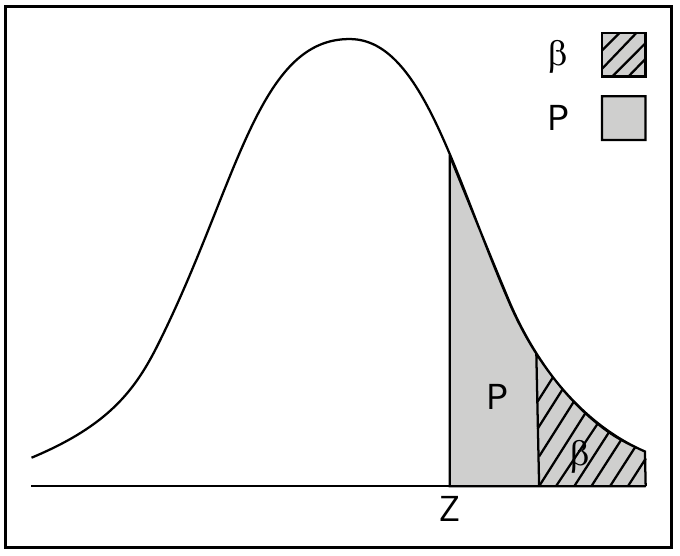
\includegraphics[height=5cm,keepaspectratio=true]{./images/kum0402.png}
	% kum0402.png: 0x0 pixel, 300dpi, 0.00x0.00 cm, bb=
	\caption{A typical normal distribution with $p$-values and significance level.}
	\label{fig:3.7.4}
\end{figure}


\subsection{Criteria}
\begin{itemize}
	\item Accept the \emph{null hypothesis and reject the alternative if $p\text{-value}>\beta$}
	\item Accept the \emph{alternative hypothesis and reject the null if $p\text{-value}<\beta$}
\end{itemize}



Due to the symmetry of the normal distribution, there are three types of hypothesis tests:
\begin{enumerate}
	\item Left-tailed;
	\item right-tailed;
	\item two-tailed.
\end{enumerate}


\subsection{Left Tail}
\begin{figure}
	\centering
	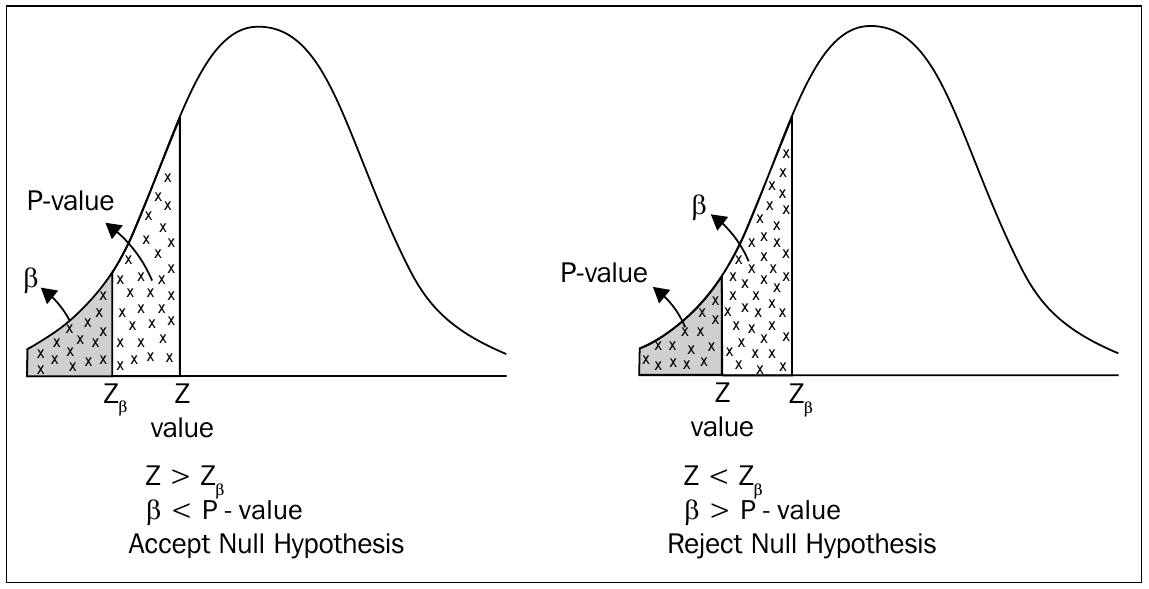
\includegraphics[width=10cm,keepaspectratio=true]{./images/kum0403.png}
	% kum0403.png: 0x0 pixel, 300dpi, 0.00x0.00 cm, bb=
	\caption{Hypothesis test: Left tail}
	\label{fig:3.7.1}
\end{figure}


\subsection{Right Tail}
\begin{figure}
	\centering
	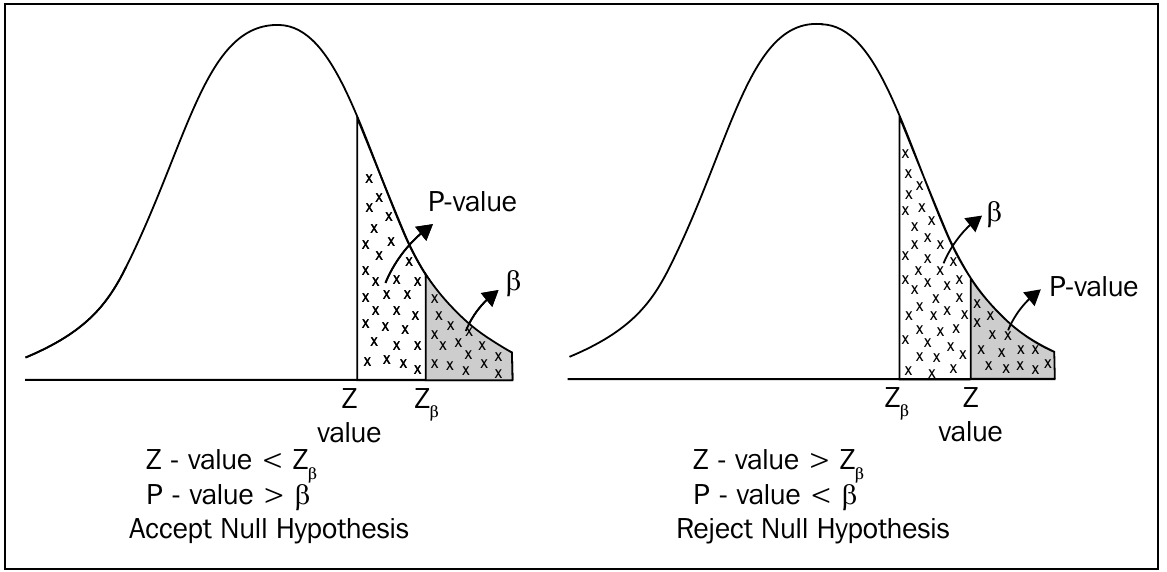
\includegraphics[width=10cm,keepaspectratio=true]{./images/kum0404.png}
	% kum0403.png: 0x0 pixel, 300dpi, 0.00x0.00 cm, bb=
	\caption{Hypothesis test: Right tail}
	\label{fig:3.7.2}
\end{figure}


\subsection{Two Tails}
We analyze both tails, and if the respective hypothesis test fails in either of the two tails, the hypothesis test is rejected.
